%% tp2.tex — Presentacion SdS TP2: automata off-lattice (Vicsek / votante)
%%
%% Compilar desde presentaciones/tp2/:  pdflatex tp2.tex   (dos veces)
%% Estilo: sdsbeamer.sty (symlink a ../sdsbeamer.sty).
%% Figuras: ../../tp2-cellular-automata/analysis/figures/  y  figuras/ (locales)
%% Animaciones: fotograma + link (el PDF de entrega no lleva video embebido).

\documentclass[aspectratio=169]{beamer}
% sdsbeamer.sty vive un directorio mas arriba. Buscarlo por \input@path en vez
% de por symlink: git no materializa symlinks en Windows (core.symlinks=false)
% y el .sty queda como un archivo de texto con la ruta adentro.
\makeatletter\def\input@path{{../}}\makeatother
\usepackage{sdsbeamer}
\usepackage{tikz}
\usetikzlibrary{arrows.meta,positioning,calc}
\microtypesetup{expansion=false}

\graphicspath{{../../tp2-cellular-automata/analysis/figures/}{figuras/}}

% Fotograma fijo representativo + enlace explicito debajo (GuiaPresentaciones 2.4.8).
% El PDF de entrega no lleva video embebido.
%   \animbox{<archivo>}{<condicion>}{<enlace>}
\newcommand{\linkpendiente}{{\color{red!70!black}[link de YouTube pendiente]}}
\newcommand{\animbox}[3]{%
  \centering
  \includegraphics[width=0.86\linewidth]{#1}\\[0.4em]
  {\small #2}\\[0.2em]
  {\scriptsize #3}%
}

\title{Autómata off-lattice: bandadas}
\subtitle{Simulación de Sistemas - ITBA}
\author[Grupo 2]{Arancibia Nicolás -- Legajo 64481 \and
  Morantes Agustín -- Legajo 61306 \and Ronda Agustín -- Legajo 64507}
\institute[ITBA]{Grupo 2 --- Comisión S2 --- Instituto Tecnológico de Buenos Aires}
\date{4 de septiembre de 2026}

\begin{document}

\begin{frame}[plain]
  \titlepage
\end{frame}

% ==========================================================================
\section{Introducción}
% Aclaración 1 del enunciado: sin sistema real; ecuaciones, sin detenerse.
% ==========================================================================

\begin{frame}{Modelo}
  \begin{block}{Vecindad y ruido}
    \begin{columns}[T,onlytextwidth]
      \begin{column}{0.48\textwidth}
        \centering
        \(
          \displaystyle
          \mathcal{N}_i(t)=\bigl\{j\neq i:
          \lvert\vect{r}_i(t)-\vect{r}_j(t)\rvert_{\mathrm{PBC}}<r_c\bigr\}
        \)
      \end{column}
      \begin{column}{0.48\textwidth}
        \centering
        \(
          \displaystyle
          \xi_i(t)\sim U[-\eta/2,\,\eta/2]
        \)
      \end{column}
    \end{columns}
  \end{block}

  \vspace{0.4em}
  \begin{columns}[T,onlytextwidth]
    \begin{column}{0.48\textwidth}
      {\color{structure}\large Vicsek}\par
      \vspace{0.55em}
      \begin{minipage}[t][0.17\textheight][t]{\linewidth}
        \centering
        \(
          \displaystyle
          \theta_i'=\arg\!\sum_{j\in\mathcal{N}_i(t)\cup\{i\}}
          e^{\mathrm{i}\theta_j(t)}+\xi_i(t)
        \)\par
        \vfill
        {\tiny Vicsek et al., PRL 1995}
      \end{minipage}
    \end{column}
    \begin{column}{0.48\textwidth}
      {\color{structure}\large Votante}\par
      \vspace{0.55em}
      \begin{minipage}[t][0.17\textheight][t]{\linewidth}
        \centering
        \(
          \displaystyle
          J_i\sim U\bigl(\mathcal{N}_i(t)\cup\{i\}\bigr),
          \qquad \theta_i'=\theta_{J_i}(t)+\xi_i(t)
        \)\par
        \vfill
        {\tiny Loscar, Baglietto y Vazquez, PRE 2021}
      \end{minipage}
    \end{column}
  \end{columns}

  \vspace{0.2em}
  \begin{block}{Movimiento y condiciones periódicas}
    \vspace{-0.55em}
    \[
      \vect{r}_i(t+\Delta t)=
      \bigl[\vect{r}_i(t)+v\,(\cos\theta_i',\,\sin\theta_i')\,\Delta t\bigr]
      \mathbin{\mathrm{mod}}\,L
    \]
  \end{block}
\end{frame}

% ==========================================================================
\section{Implementación}
% Solo el motor. Sin post-proceso ni I/O.
% ==========================================================================

\begin{frame}{Motor}
  \centering
  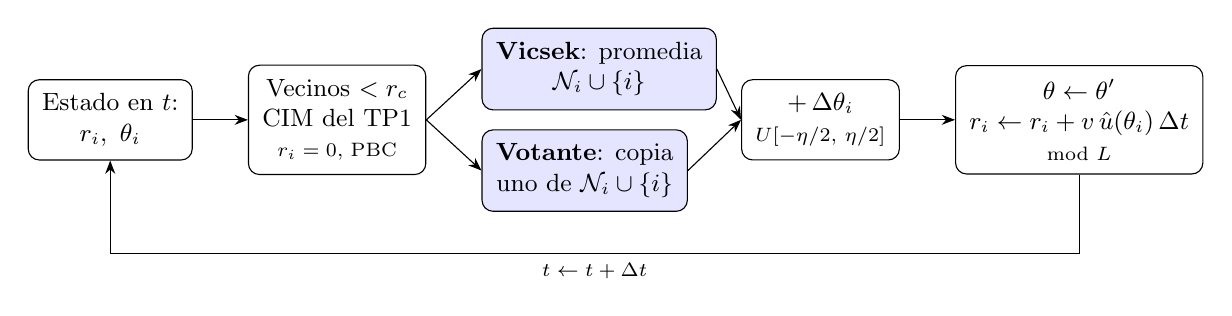
\begin{tikzpicture}[>=Stealth, font=\small,
      caja/.style={draw, rounded corners, align=center, inner sep=5pt},
      regla/.style={caja, fill=blue!10}]
    \node[caja] (estado) {Estado en $t$:\\ $\vect{r}_i,\ \theta_i$};
    \node[caja, right=0.7cm of estado] (cim) {Vecinos $< r_c$\\ CIM del TP1\\ {\scriptsize $r_i = 0$, PBC}};
    \node[regla, above right=0.12cm and 0.7cm of cim.east, anchor=south west] (vicsek)
      {\textbf{Vicsek}: promedia\\ $\mathcal{N}_i \cup \{i\}$};
    \node[regla, below right=0.12cm and 0.7cm of cim.east, anchor=north west] (voter)
      {\textbf{Votante}: copia\\ uno de $\mathcal{N}_i \cup \{i\}$};
    \node[caja] (ruido) at ($(vicsek.east)!0.5!(voter.east) + (1.5,0)$)
      {$+\,\Delta\theta_i$\\ {\scriptsize $U[-\eta/2,\,\eta/2]$}};
    \node[caja, right=0.7cm of ruido] (mover)
      {$\theta \leftarrow \theta'$\\ $\vect{r}_i \leftarrow \vect{r}_i + v\,\hat{\vect{u}}(\theta_i)\,\Delta t$\\ {\scriptsize mod $L$}};
    \draw[->] (estado) -- (cim);
    \draw[->] (cim.east) -- (vicsek.west);
    \draw[->] (cim.east) -- (voter.west);
    \draw[->] (vicsek.east) -- (ruido.west);
    \draw[->] (voter.east) -- (ruido.west);
    \draw[->] (ruido) -- (mover);
    \draw[->] (mover.south) -- ++(0,-1.0) -| (estado.south)
      node[pos=0.25, below, font=\scriptsize] {$t \leftarrow t + \Delta t$};
  \end{tikzpicture}

  \vspace{0.7em}
  \begin{itemize}
    \item Java. Dos buffers de $\theta$: la regla lee $\theta(t)$, nunca $\theta'$ (sincrónico).
    \item Sin vecinos, ambas reglas conservan la dirección propia ($+$ ruido).
    \item Clusters para $S$: union-find sobre la misma lista de vecinos del CIM.
  \end{itemize}
\end{frame}

% ==========================================================================
\section{Simulaciones}
% ==========================================================================

\begin{frame}{Sistema}
  \begin{columns}[c]
    \begin{column}{0.38\textwidth}
      \centering
      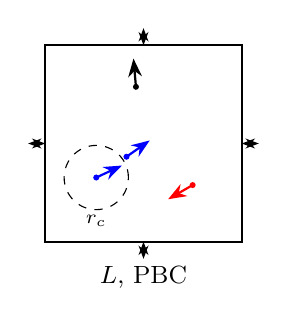
\begin{tikzpicture}[scale=0.48, >=Stealth]
        \draw[thick] (0,0) rectangle (5.2,5.2);
        \draw[<->, dashed] (-0.45,2.6) -- (0,2.6);
        \draw[<->, dashed] (5.2,2.6) -- (5.65,2.6);
        \draw[<->, dashed] (2.6,-0.45) -- (2.6,0);
        \draw[<->, dashed] (2.6,5.2) -- (2.6,5.65);
        \draw[dashed] (1.35,1.7) circle (0.85);
        \fill[blue] (1.35,1.7) circle (0.08);
        \draw[->, thick, blue] (1.35,1.7) -- ++(25:0.75);
        \fill[blue] (2.15,2.25) circle (0.08);
        \draw[->, thick, blue] (2.15,2.25) -- ++(35:0.75);
        \fill[red] (3.9,1.5) circle (0.08);
        \draw[->, thick, red] (3.9,1.5) -- ++(210:0.75);
        \fill[black] (2.4,4.1) circle (0.08);
        \draw[->, thick, black] (2.4,4.1) -- ++(95:0.75);
        \node[font=\scriptsize] at (1.35,0.55) {$r_c$};
        \node[font=\small] at (2.6,-0.95) {$L$, PBC};
      \end{tikzpicture}
    \end{column}
    \begin{column}{0.60\textwidth}
      \textbf{Fijos}
      \begin{itemize}
        \item $L = 10\uni{m}$, PBC, $r_c = 1\uni{m}$
        \item $v = 0.03\uni{m/s}$, $\Delta t = 1\uni{s}$
        \item Partículas puntuales
      \end{itemize}
      \textbf{Variables}
      \begin{itemize}
        \item Modelo: Vicsek o votante
        \item $\rho = 2,\,4,\,8$ ($N = 200,\,400,\,800$)
        \item $\eta \in [0,\,2\pi]\uni{rad}$
      \end{itemize}
      \textbf{Extra} (para $S$): $\rho = 1/(3\pi),\,1/(2\pi),\,1/\pi$
      \newline{\small $N = 11,\,16,\,32$; $\langle k \rangle = \rho\pi r_c^2 < 1$}
    \end{column}
  \end{columns}
\end{frame}

\begin{frame}{Observables}
  Del estado $(\vect{r}_i,\,\vect{v}_i)$ en cada paso:
  \begin{equation*}
    v_a(t) = \frac{1}{Nv}\left\lvert\sum_{i=1}^{N}\vect{v}_i(t)\right\rvert,
    \qquad
    S(t) = \frac{1}{N}\max_c \lvert c \rvert
  \end{equation*}
  $c$ = componente conexa del grafo de vecindad (arista si distancia $< r_c$).

  \vspace{0.4em}
  Escalar de cada corrida: promedio temporal sobre la segunda mitad
  ($t \ge T/2$, con $T$ la duración total), ya dentro del estacionario.
  \begin{itemize}
    \item $T = 2000$ pasos ($5000$ si $\rho < 2$)
    \item 50 seeds distintas por punto $(\mathrm{modelo},\,\rho,\,\eta)$
    \item Punto en las curvas: media entre seeds. Barra: desvío muestral
  \end{itemize}
\end{frame}

% ==========================================================================
\section{Resultados}
% Por estudio: animacion -> evolucion -> input vs observable.
% Recorte: ρ=4 como caso típico; ρ=2,4,8 en las curvas; densidades bajas
% solo donde S deja de ser trivial.
% ==========================================================================

\begin{frame}{Vicsek: animación}
  \begin{columns}[c,onlytextwidth]
    \begin{column}{0.70\textwidth}
      \begin{columns}[T,onlytextwidth]
        \begin{column}{0.5\textwidth}
          \animbox{anim_vicsek_rho4_eta05.png}{$\eta = 0.5\uni{rad}$, $v_a = 0.99$}{\linkpendiente}
        \end{column}
        \begin{column}{0.5\textwidth}
          \animbox{anim_vicsek_rho4_eta4.png}{$\eta = 4\uni{rad}$, $v_a = 0.18$}{\linkpendiente}
        \end{column}
      \end{columns}
    \end{column}
    \begin{column}{0.28\textwidth}
      {\small Vicsek, $\rho = 4$ ($N = 400$) \\[0.35em]
      Vectores $=$ velocidad, color $=$ ángulo. \\[0.35em]
      Fotograma en $t = 1500\uni{s}$. \\[0.35em]
      $L = 10\uni{m}$, $r_c = 1\uni{m}$,
      $v = 0.03\uni{m/s}$, $\Delta t = 1\uni{s}$.}
    \end{column}
  \end{columns}
\end{frame}

\begin{frame}{Vicsek: $v_a(t)$}
  \figuraparam{evolucion_va_vicsek_rho4.png}{%
    Vicsek, $\rho = 4$, corrida típica \\[0.35em]
    Menos ruido $\to$ ordena antes y satura más alto.
  }
\end{frame}

\begin{frame}{Vicsek: $v_a$ vs $\eta$}
  \figuraparam{vicsek_va_vs_eta.png}{%
    Vicsek, 50 seeds \\[0.35em]
    De orden total sin ruido a desorden con $\eta$ alto. \\[0.35em]
    Mayor $\rho$ corre la caída hacia $\eta$ más alto.
  }
\end{frame}

\begin{frame}{Vicsek: $S(t)$}
  \figuraparam{evolucion_s_vicsek_rho2.png}{%
    Vicsek, $\rho = 2$, corrida típica \\[0.35em]
    Eje acotado: todas las curvas viven cerca de 1. \\[0.35em]
    Con $\rho \ge 2$ el grafo de vecinos percola: el cluster más grande abarca casi todo el sistema, con o sin ruido.
  }
\end{frame}

\begin{frame}{Vicsek: $S$ vs $\eta$}
  \figuraparam{vicsek_s_vs_eta.png}{%
    Vicsek \\[0.35em]
    $\rho = 2,\,4,\,8$: el cluster más grande toma casi la totalidad de las partículas, sin importar el ruido. \\[0.35em]
    $\rho \le 1/\pi$: $S$ cae con $\eta$ y se aplana a partir de $\eta \approx 4\uni{rad}$, en las tres densidades bajas.
  }
\end{frame}

\begin{frame}{Vicsek: $v_a$ vs $S$}
  \centering
  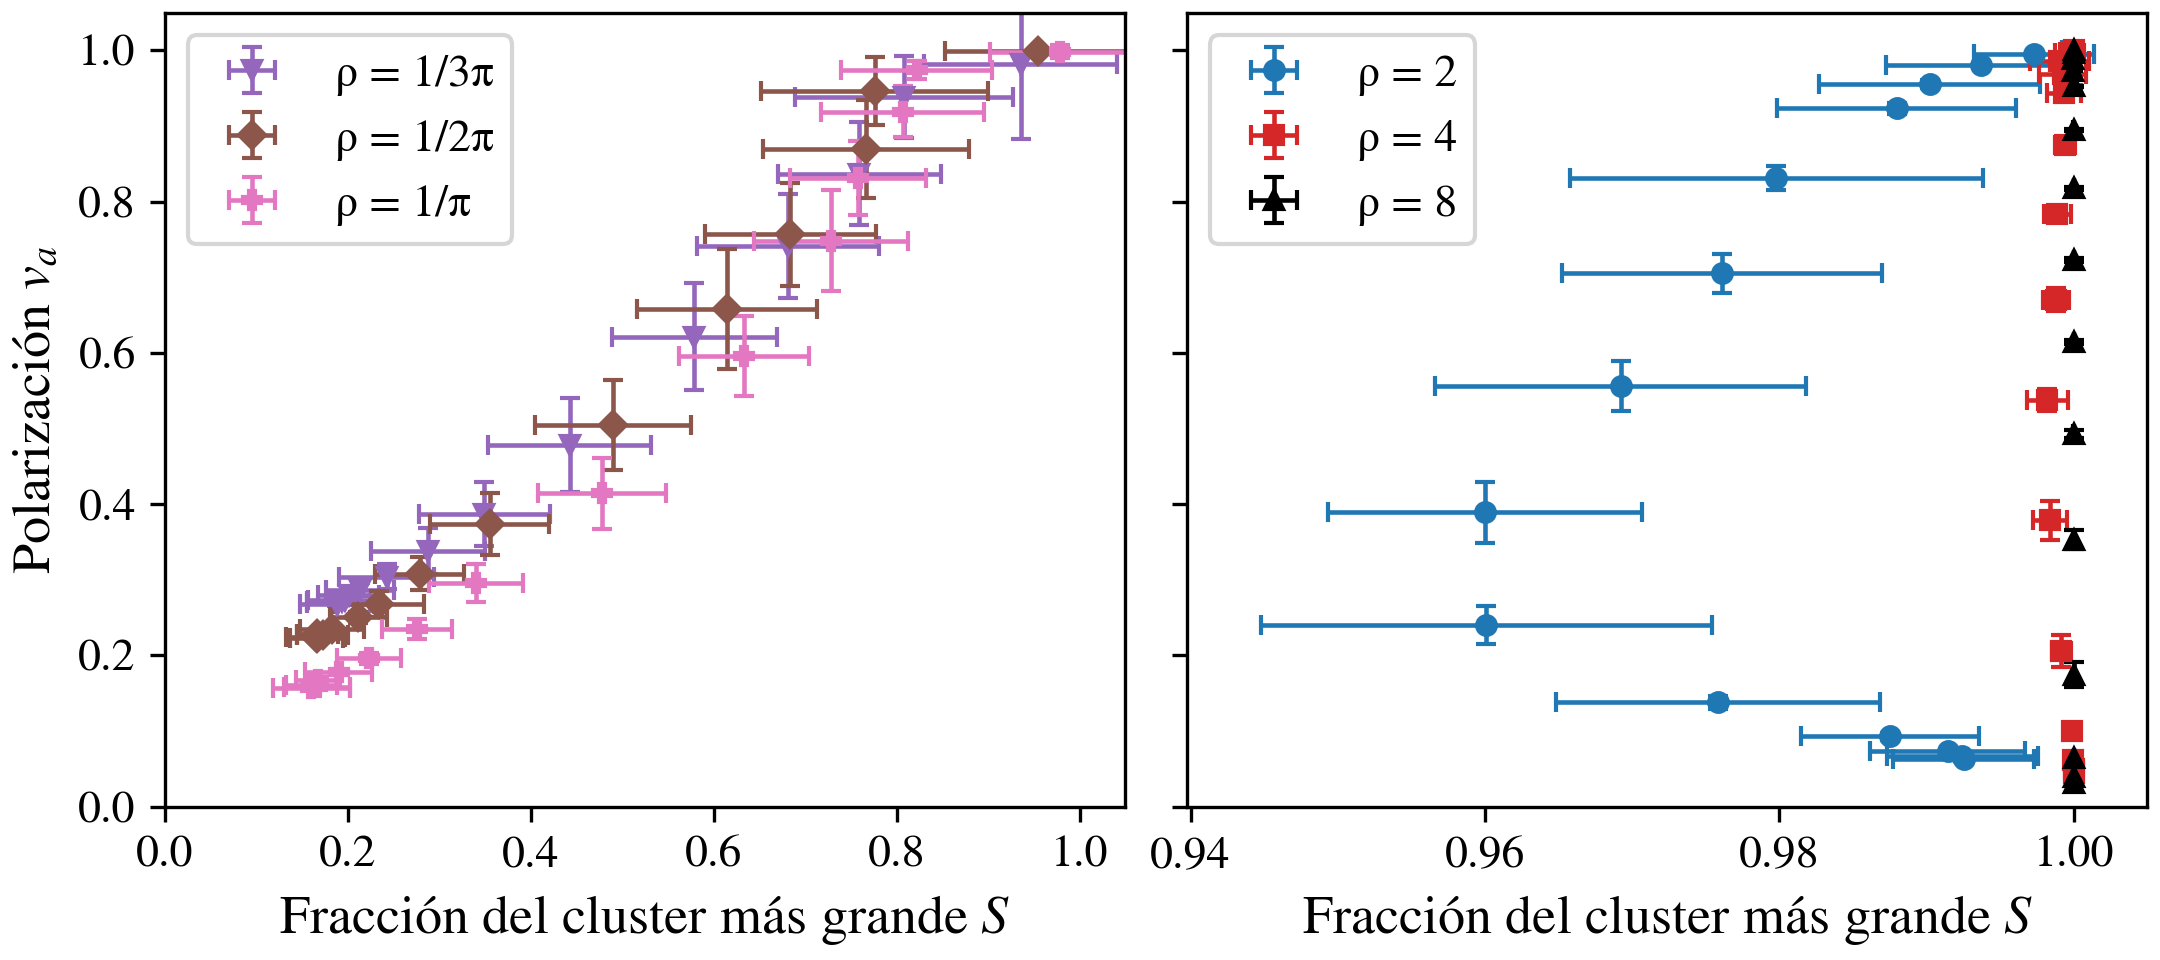
\includegraphics[width=0.84\linewidth]{va_vs_s_vicsek.png}

  \vspace{0.3em}
  {\small Vicsek, 50 seeds. Cada punto: un $\eta$. Paneles con distinta escala en $S$:
  a la izquierda $v_a$ crece con $S$ (el orden necesita conectividad), a la derecha
  $S$ no se mueve mientras $v_a$ recorre todo su rango.}
\end{frame}

\begin{frame}{Votante: animación}
  \begin{columns}[c,onlytextwidth]
    \begin{column}{0.70\textwidth}
      \begin{columns}[T,onlytextwidth]
        \begin{column}{0.5\textwidth}
          \animbox{anim_voter_rho4_eta05.png}{$\eta = 0.5\uni{rad}$, $v_a = 0.45$}{\linkpendiente}
        \end{column}
        \begin{column}{0.5\textwidth}
          \animbox{anim_voter_rho4_eta4.png}{$\eta = 4\uni{rad}$, $v_a = 0.08$}{\linkpendiente}
        \end{column}
      \end{columns}
    \end{column}
    \begin{column}{0.28\textwidth}
      {\small Votante, $\rho = 4$ ($N = 400$) \\[0.35em]
      Mismos ruidos, mismo instante y misma representación que Vicsek. \\[0.35em]
      A $\eta = 0.5\uni{rad}$ Vicsek está en $v_a = 0.99$ y el votante ya
      recorre todo el círculo.}
    \end{column}
  \end{columns}
\end{frame}

\begin{frame}{Votante: $v_a(t)$}
  \figuraparam{evolucion_va_voter_rho4.png}{%
    Votante, $\rho = 4$, corrida típica \\[0.35em]
    $\eta = 0$: ordena y satura en 1. \\[0.35em]
    $\eta = 0.5\uni{rad}$: deriva sin estacionarse (por eso no lleva recta vertical). \\[0.35em]
    $\eta = 2\uni{rad}$: desorden desde el inicio.
  }
\end{frame}

\begin{frame}{Votante: $v_a$ vs $\eta$}
  \figuraparam{voter_va_vs_eta.png}{%
    Votante, 50 seeds \\[0.35em]
    Todas las densidades pierden el orden dentro del primer radián. \\[0.35em]
    A diferencia de Vicsek, subir $\rho$ no corre la caída.
  }
\end{frame}

\begin{frame}{Vicsek vs votante: $v_a$ vs $\eta$}
  \figuraparam{comparacion_va_vs_eta_rho4.png}{%
    $\rho = 4$, 50 seeds \\[0.35em]
    Sin ruido, ambos alcanzan $v_a = 1$. \\[0.35em]
    El votante pierde el orden con ruidos mucho menores: promediar filtra el ruido, copiar a uno solo no. \\[0.35em]
    Misma forma en $\rho = 2$ y $8$.
  }
\end{frame}

\begin{frame}{Votante: $S(t)$}
  \figuraparam{evolucion_s_voter_rho2.png}{%
    Votante, $\rho = 2$, corrida típica \\[0.35em]
    Eje acotado: todas las curvas viven cerca de 1. \\[0.35em]
    Mismo comportamiento que Vicsek: con $\rho \ge 2$ el grafo de vecinos percola y el cluster más grande abarca casi todo, con o sin ruido.
  }
\end{frame}

\begin{frame}{Votante: $S$ vs $\eta$}
  \figuraparam{voter_s_vs_eta.png}{%
    Votante \\[0.35em]
    Igual que en Vicsek: $\rho \ge 2$ percola, $\rho \le 1/\pi$ cae con $\eta$. \\[0.35em]
    La conectividad depende de la densidad, no de la regla de alineación.
  }
\end{frame}

\begin{frame}{Votante: $v_a$ vs $S$}
  \centering
  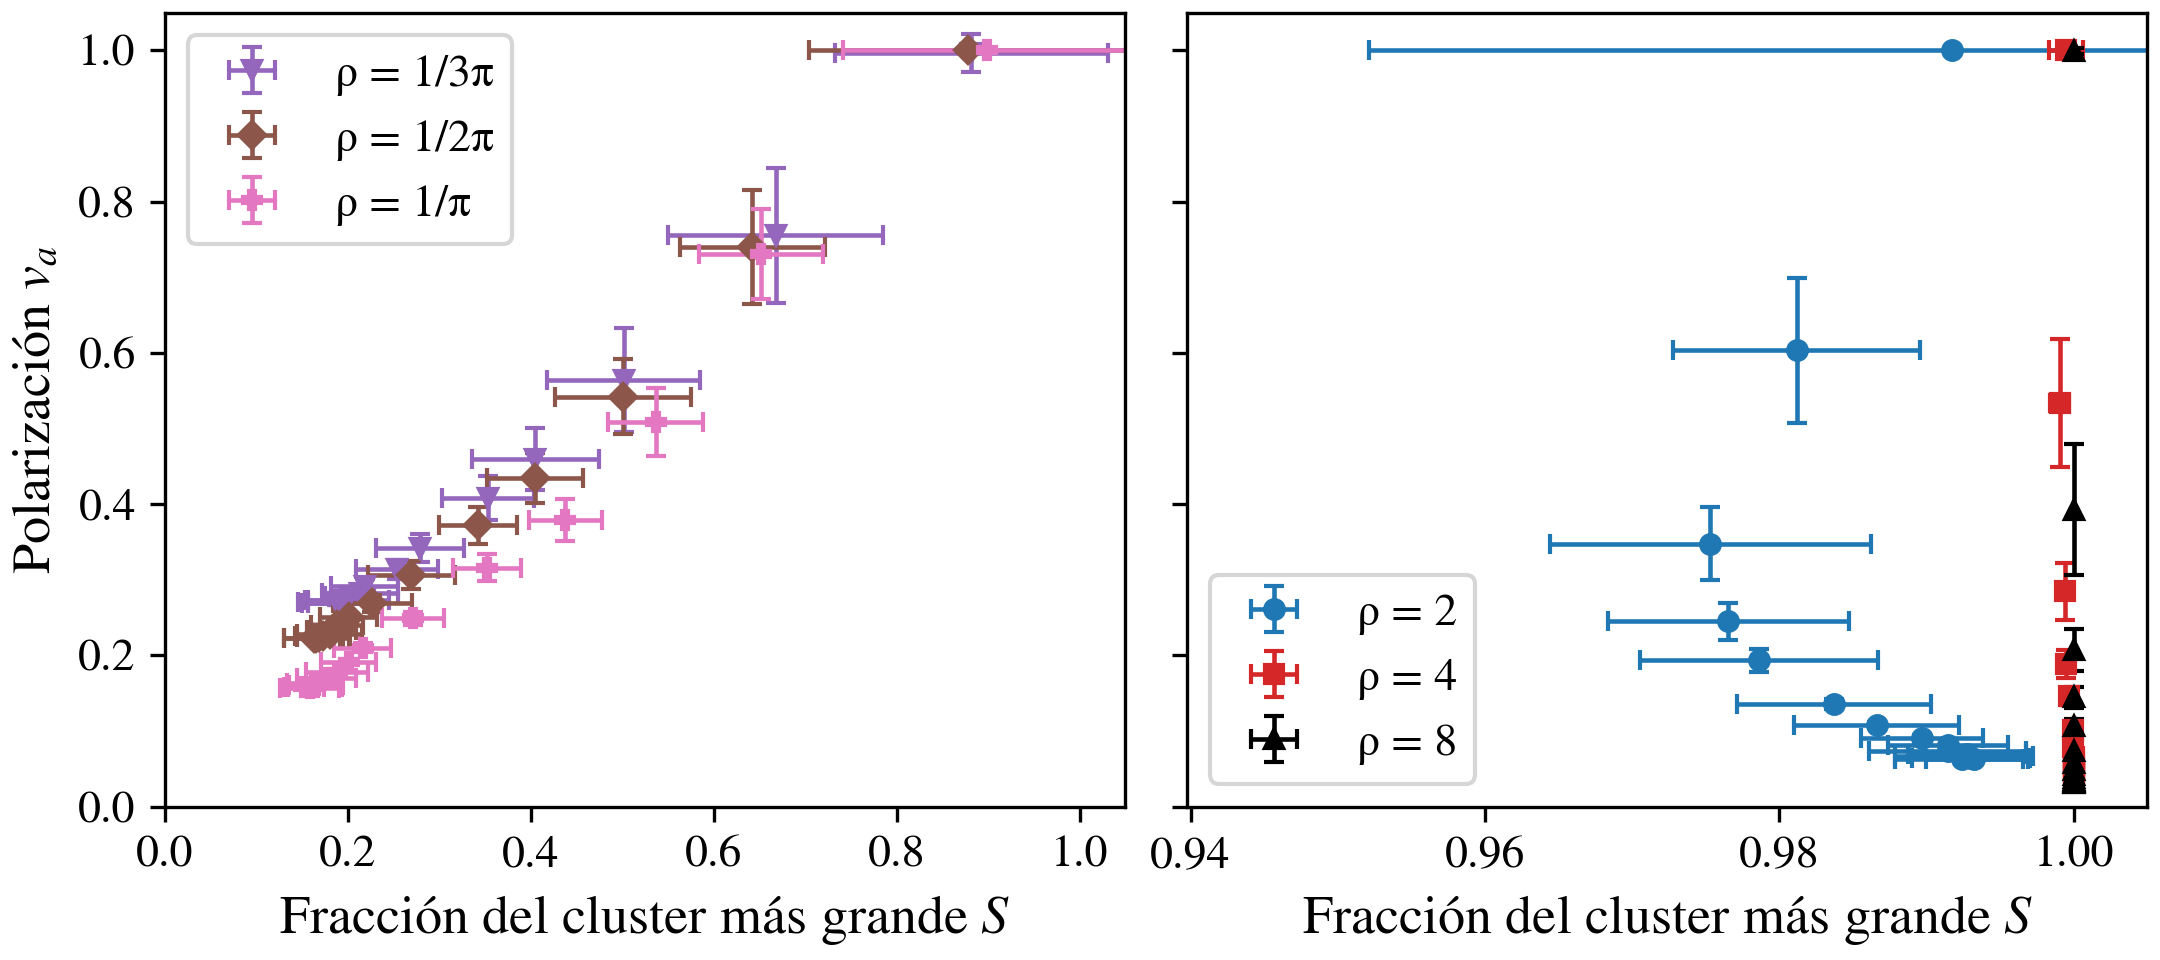
\includegraphics[width=0.84\linewidth]{va_vs_s_voter.png}

  \vspace{0.3em}
  {\small Votante, 50 seeds. Misma estructura que Vicsek: correlación a la izquierda,
  columna en $S \approx 1$ a la derecha. La conectividad no depende de la regla.}
\end{frame}

\begin{frame}{Vicsek vs votante: $S$ vs $\eta$}
  \figuraparam{comparacion_s_vs_eta_rho4.png}{%
    $\rho = 4$, 50 seeds \\[0.35em]
    Ojo con el eje: está acotado a los datos. Mínimos $0.9982$ y $0.9991$, toda
    la variación entra en menos del $0.2\%$. \\[0.35em]
    La regla de alineación separa $v_a$ en un factor tres, pero no deja huella
    en la conectividad.
  }
\end{frame}

\begin{frame}{Vicsek vs votante: $v_a$ vs $S$}
  \centering
  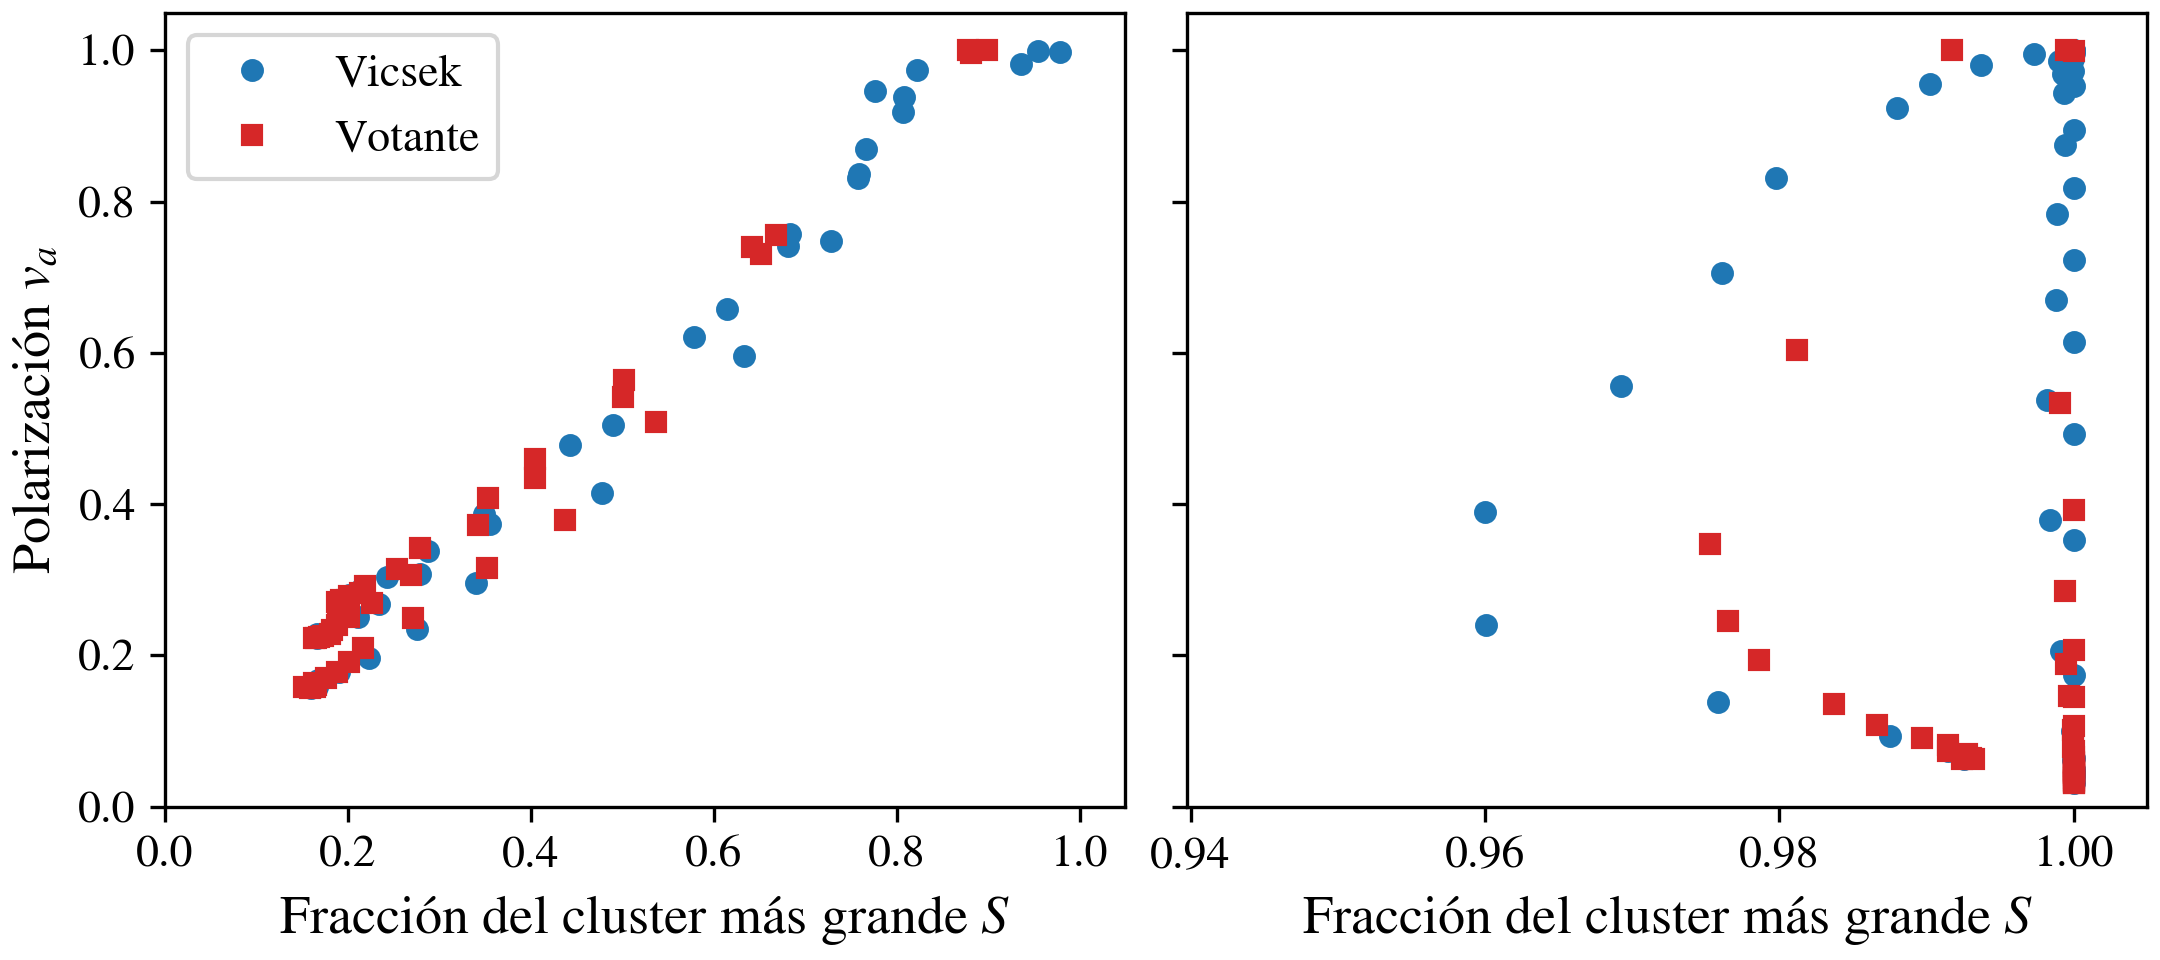
\includegraphics[width=0.84\linewidth]{comparacion_va_vs_s.png}

  \vspace{0.3em}
  {\small Cada panel junta las tres densidades de su grupo. A la izquierda las dos
  nubes se solapan: con menos de un vecino por partícula, promediar y copiar dejan de
  distinguirse. A la derecha ambos modelos se apilan en $S \approx 1$.
  $S$ no separa una regla de la otra en ningún régimen.}
\end{frame}

\begin{frame}{Tiempos del CIM}
  \figuraparam{cim_tp1_vs_tp2.png}{%
    Misma geometría que el TP1: $L = 10\uni{m}$, $M = 10$, $r_c = 1\uni{m}$, PBC, partículas puntuales
  }
\end{frame}

% ==========================================================================
\section{Conclusiones}
% Solo lo que está en las figuras de Resultados.
% ==========================================================================

\begin{frame}{Conclusiones}
  \begin{itemize}
    \item Vicsek es mucho más robusto al ruido que el votante: con $\rho = 4$ y
      $\eta = 2\uni{rad}$, $\langle v_a \rangle \approx 0.8$ contra $\approx 0.1$;
      ya con $\eta = 0.5\uni{rad}$ el votante cae a $0.29 \pm 0.04$
      mientras Vicsek sigue en $0.99$.
    \item La densidad determina el tamaño del cluster más grande: con $\rho = 2,\,4,\,8$,
      $S$ se mantiene $\approx 1$ para todo ruido;
      con $\rho \le 1/\pi$ queda lejos de 1.
    \item En densidades bajas, a mayor ruido menor es el $S$ estacionario:
      cae de $\approx 0.95$ a $\approx 0.2$ recorriendo $\eta$.
  \end{itemize}
\end{frame}

\begin{frame}[plain]
  \centering
  \vfill
  {\Huge Muchas gracias}
  \vfill
\end{frame}

\end{document}
